\chapter{Конструкторский раздел}\label{sec:design}

В данном разделе будут формализованы сущности системы, описана конкретная ролевая модель, спроектировано приложение, взаимодействующее с базой данных, выбрана конкретная СУБД, а также спроектирован триггер.

\section{Выбор СУБД}

На основе анализа различных моделей данных, сделанного в предыдущем разделе, выдвинутых требований к приложению и формализованных данных в качестве используемой СУБД был выбран PostgreSQL \cite{postgres}, поскольку он является объектно-реляционной СУБД \cite{postgresdocs}, что позволяет пользоваться основными достоинствами объектно-ориентированной модели данных и простотой структуры реляционных моделей, а также обладает достаточным набором инструментов для решения поставленной задачи.

\section{Формализация сущностей системы}

На основе сущностей, выделенных выше, были спроектированы следующие таблицы.

\begin{enumerate}
	\item Таблица competitions, содержащая информацию о турнирах, имеет следующие поля:
	\begin{itemize}
		\item id --- идентификатор соревнования, целочисленный тип;
		\item name --- название соревнования символьный тип;
		\item dt --- дата турнира, тип дата;
		\item ageCategory --- возрастная категория, символьный тип;
		\item weaponType --- оружие, символьный тип;
		\item sex --- пол, символьный тип;
		\item isTeam --- является ли соревнование командным, логический тип;
		\item status --- статус соревнований, символьный тип;
		\item numOfAthlets --- число участников, целочисленный тип.
	\end{itemize}
	\item Таблица account, содержащая общую информацию об аккаунте, имеет следующие поля:
	\begin{itemize}
		\item id --- идентификатор соревнования, целочисленный тип;
		\item name --- ФИО пользователя, символьный тип;
		\item birthday --- дата рождения, тип дата;
		\item sex --- пол, символьный тип;
		\item email --- адрес электронной почты, уникальное поле, символьный тип.
	\end{itemize}
	\item Таблица athlet, хранящая информацию о спортсмене, имеет следующие поля:
	\begin{itemize}
		\item IDFFR --- номер Федерации фехтования России, является идентификатором, целочисленный тип;
		\item IDAccount --- идентификатор соответствующего аккаунта, целочисленный тип;
		\item hand --- вооруженная рука, символьный тип;
		\item insurance --- наличие страховки, логический тип;
		\item license --- наличие лицензии, логический тип;
		\item weaponType --- оружие, символьный тип;
		\item rank --- разряд, символьный тип.
	\end{itemize}
	\item Таблица battles, содержащая информацию о проведенном бою, имеет следующие поля: 
	\begin{itemize}
		\item id --- идентификатор боя, целочисленный тип;
		\item idWinner --- идентификатор победителя, целочисленный тип;
		\item idLooser --- идентификатор проигравшего, целочисленный тип;
		\item idCompetition --- идентификатор соревнования, целочисленный тип;
		\item scoreWinner --- счет победителя, целочисленный тип;
		\item scoreLooser --- счет проигравшего, целочисленный тип.
	\end{itemize}
	\item Таблица users, хранящая информацию о зарегистрированных пользователях, имеет следующие поля:
	\begin{itemize}
		\item email --- адрес электронной почты, является идентификатором, символьный тип;
		\item password --- хешированный пароль, символьный тип;
		\item role --- роль, символьный тип;
		\item verified --- статус подтверждения роли.
	\end{itemize}
	\item Таблица AthletComp, содержащая информацию о заявках спортсменов на турниры, имеет следующие поля:
	\begin{itemize}
		\item id --- идентификатор заявки, целочисленный тип;
		\item idCompetition --- идентификатор турнира, целочисленный тип;
		\item email --- адрес электронной почты пользователя, который отправил заявку, целочисленный тип.
	\end{itemize}
\end{enumerate}

Соответствующая диаграмма по описанным выше данным представлена на рисунке \ref{ris:erdb}.

\begin{figure}[H]
	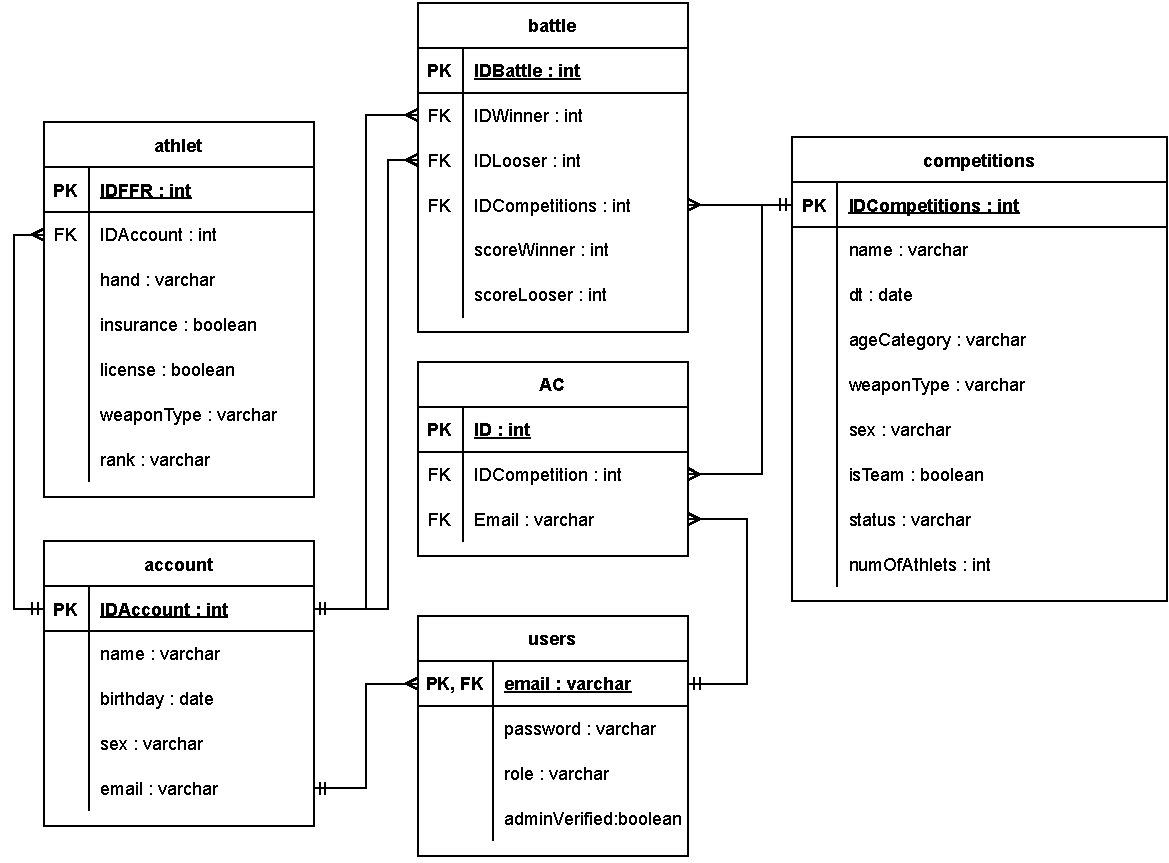
\includegraphics[width=1\columnwidth]{assets/erdb.drawio.pdf}
	\centering
	\caption{ER-диаграмма системы}
	\label{ris:erdb}
\end{figure}

\section{Ролевая модель}

На уровне базы данных выделена следующая ролевая модель:

\begin{enumerate}
	\item Guest --- гость. Обладает правами:
	\begin{itemize}
		\item SELECT над таблицей competitions;
		\item INSERT над таблицей users.
	\end{itemize}
	\item User --- пользователь. Обладает правами:
	\begin{itemize}
		\item INSERT/DELETE/SELECT над таблицей AyhletComp;
		\item INSERT над таблицей users;
		\item SELECT над таблицей competitions;
		\item SELECT над таблицей account.
	\end{itemize}
	\item Administrator --- администратор. Обладает правами:
	\begin{itemize}
		\item INSERT/DELETE/SELECT над таблицей AyhletComp;
		\item всеми правами над таблицей users;
		\item всеми правами над таблицей competitions;
		\item всеми правами над таблицей battles;
		\item всеми правами над таблицей athlets.
	\end{itemize}
\end{enumerate}

\section{Триггер}

В системе предусмотрен автоматический подсчет участников каждого турнира. Он реализован с помощью двух триггеров:

\begin{itemize}
	\item триггера BEFORE на действие INSERT в таблицу AthletComp, которая хранит в себе заявки спортсменов на интересующие их турниры;
	\item триггера AFTER на действие DELETE в таблице AthletComp.
\end{itemize}

Данные триггеры увеличивают или уменьшают значение поля numOfAthlets, которое хранит число участников, таблицы competitions соответственно.

На рисунке \ref{ris:trigger-delete} представлена схема работы триггера DecNum().

\begin{figure}[H]
	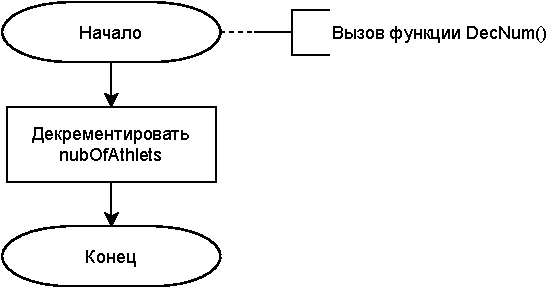
\includegraphics[width=0.5\columnwidth]{assets/trigger-delete.pdf}
	\centering
	\caption{Триггер AFTER на удаление заявки}
	\label{ris:trigger-delete}
\end{figure}

На рисунке \ref{ris:trigger-insert} представлена схема алгоритма работы триггера функции updateNum().

\begin{figure}[H]
		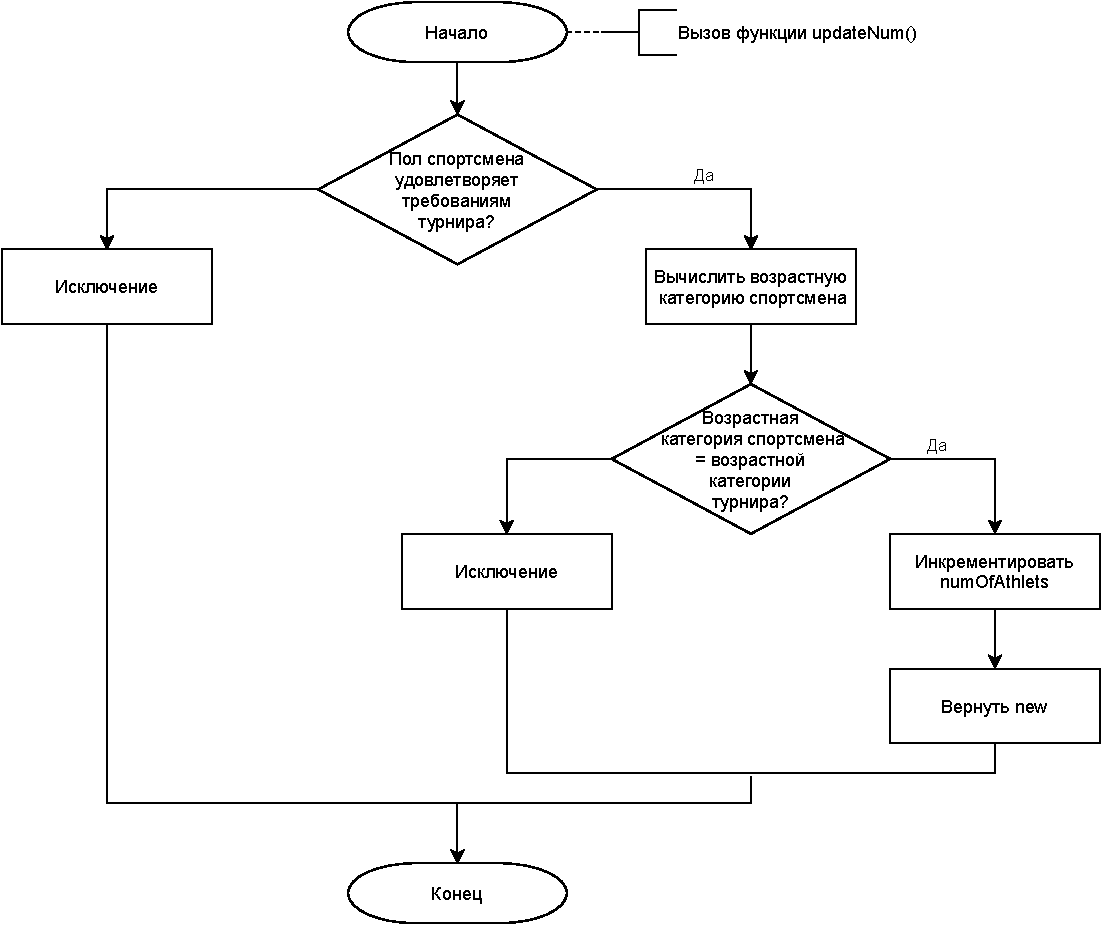
\includegraphics[width=0.8\columnwidth]{assets/trigger-insert.pdf}
	\centering
	\caption{Триггер BEFORE на создание новой заявки}
	\label{ris:trigger-insert}
\end{figure}

\section{Проектирование приложения}

Программа, осуществляющая взаимодействие с базой данных, представляет собой веб-приложение. Разработка будет осуществляться по принципам <<чистой архитектуры>>, что позволит выделить следующие компоненты: бизнес-логика, доступ к данным, транспортный слой.

%Также были выделены следующие сущности системы, представленные на рисунке \ref{ris:entity}.
%
%\begin{figure}[H]
%		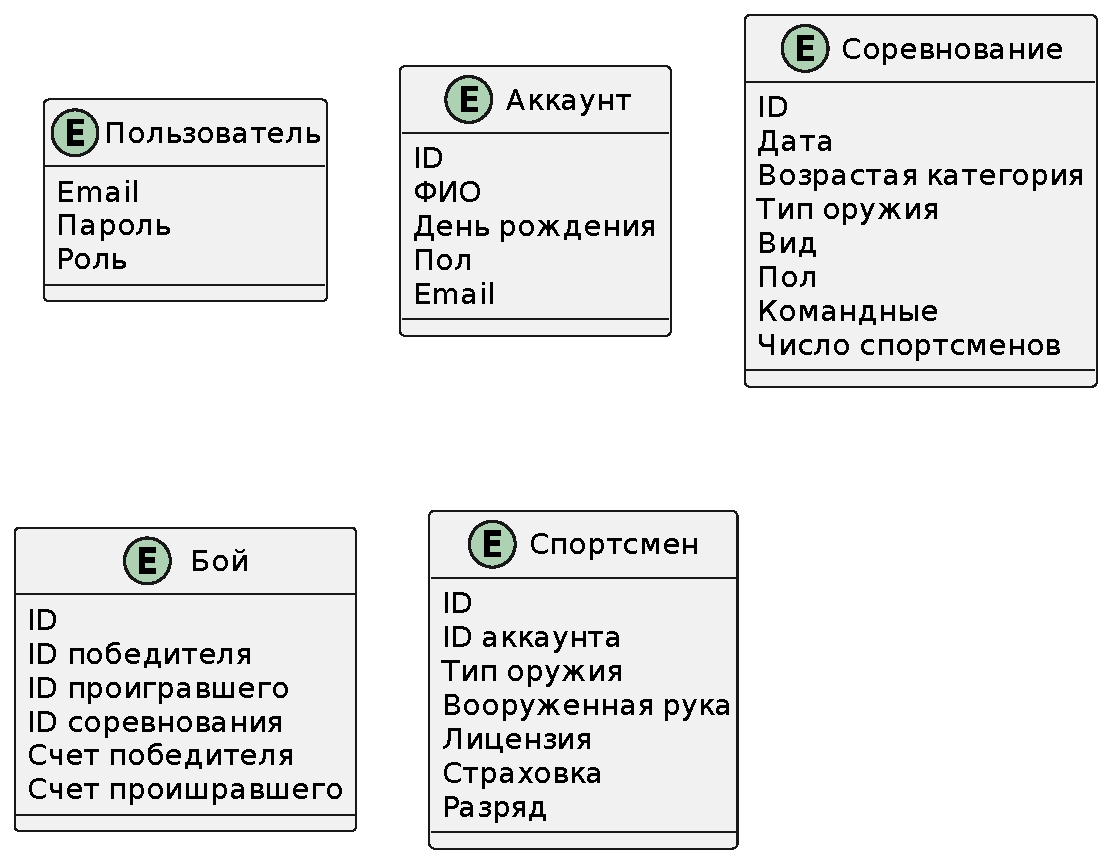
\includegraphics[width=1\columnwidth]{assets/out/entiry/entities.pdf}
%	\centering
%	\caption{Сущности системы}
%	\label{ris:entity}
%\end{figure}

\section{Вывод}

В данном разделе была выбрана конкретная СУБД, спроектирована база данных: выделено 3 типа ролей, спроектированы триггеры и общая схема базы данных.
%\section{Проектирование базы данных}
%
%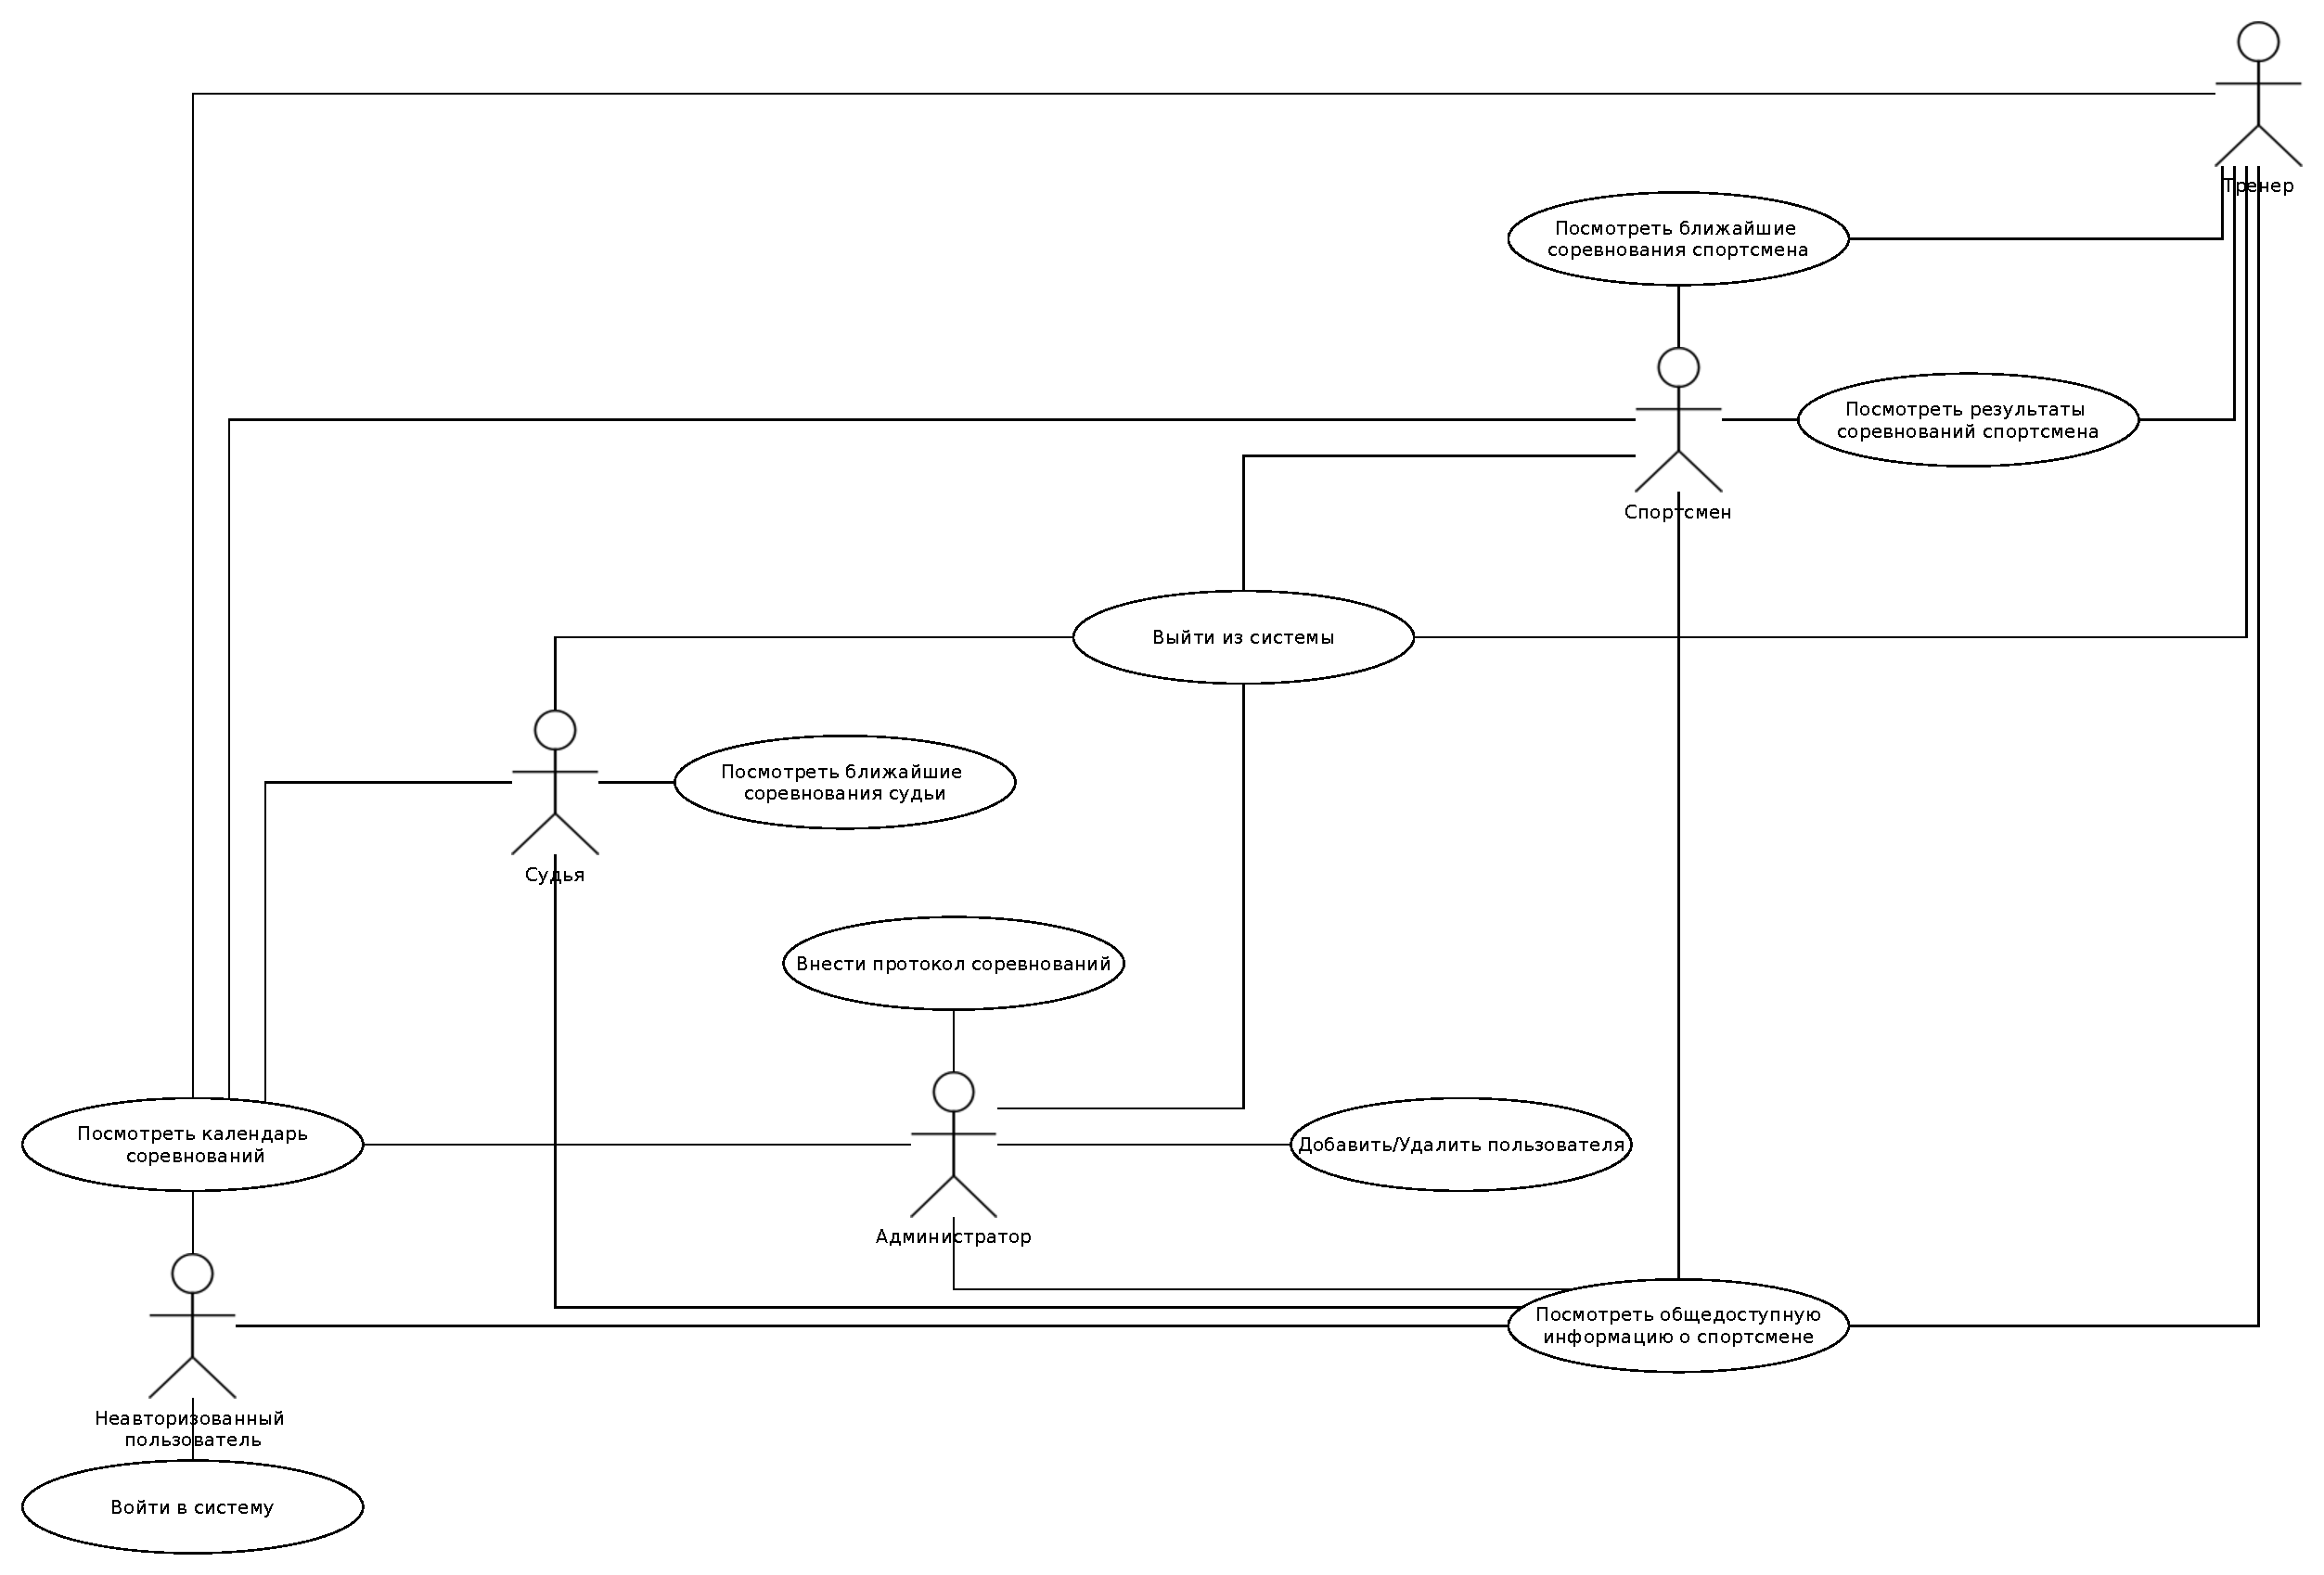
\includegraphics[width=1\columnwidth]{assets/usecase.pdf}
%
%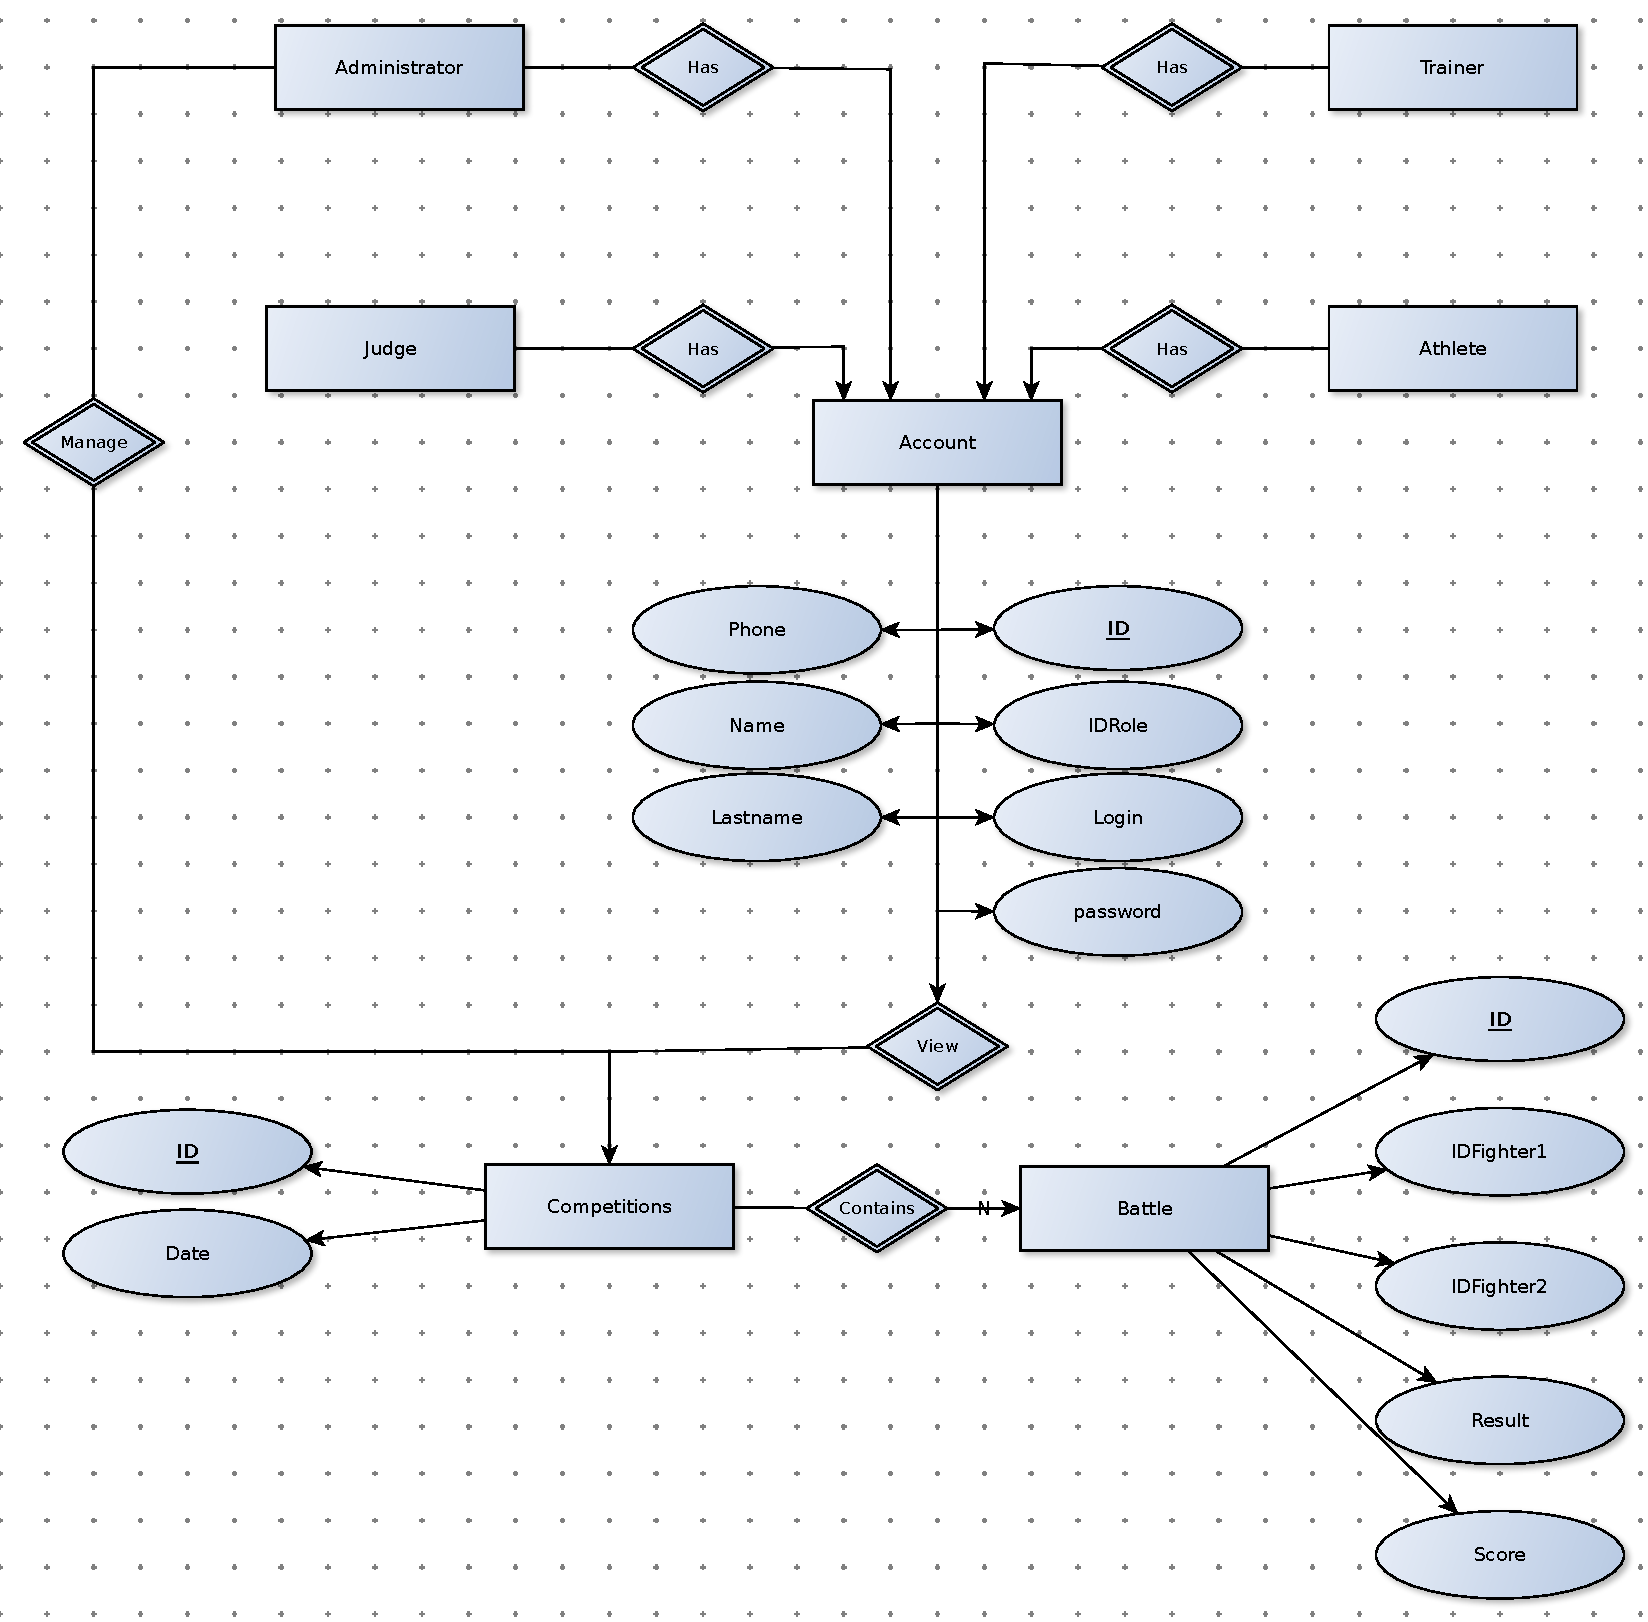
\includegraphics[width=1\columnwidth]{assets/er.pdf}
%
%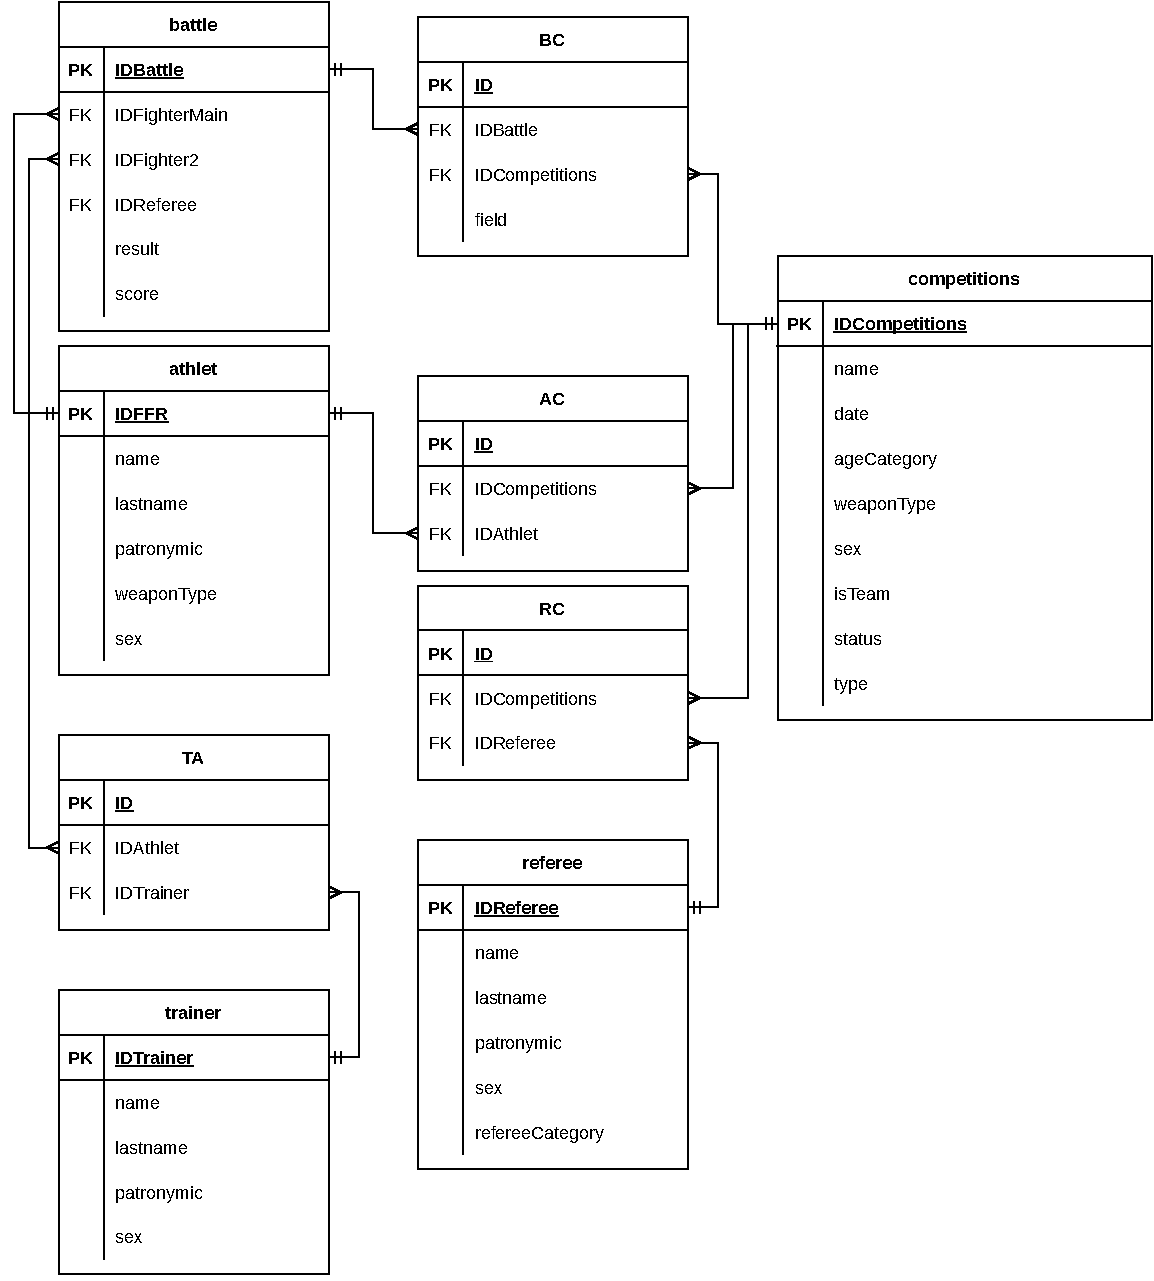
\includegraphics[width=1\columnwidth]{assets/erdb.pdf}
%
%\section{Требования к программе}
%
%\section{Проектирование приложения}
%
%\section{Вывод}